\section*{TELNET (Telecommunication Network)}
Es uno de los protocolos mas antiguos de Internet, data de la época del ARPANET y se utiliza para conectar con un equipo remoto a través de la red, de forma que el ordenador cliente se comporta como una terminal conectada con el remoto. Todo lo que se necesita es un cliente Telnet.
\subsection*{Funcionamiento}
Está basado en tres ideas:\\
\begin{itemize}
\item El concepto de \textbf{NVT (Network Virtual Terminal)}. Una NVT es un dispositivo imaginario que posee una estructura básica comun a una amplia gamma de terminales reales. Cada host mapea las características de su propia terminal sobre las de su correspondiente NVT.
\item Una perspectiva simétrica de las terminales y los procesos.
\item Negociación de las opciones de la terminal. El protocolo usa el principio de opciones negociadas ya que muchos host pueden desear suministrar servicios adicionales, mas alla de la disponible en la NVT.
\end{itemize}
\subsection*{Estructura de comandos TELNET}
La comunicación entre cliente y servidor es manejada por comandos internos, que son accesibles a los usuarios. Todos los comandos internos de \texttt{TELNET} consisten en secuencias de dos o tres bytes, dependiendo del tipo de comando:

\begin{center}
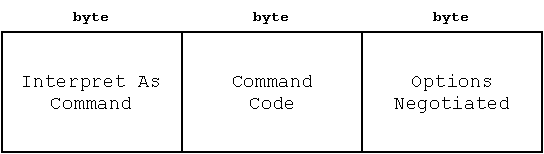
\includegraphics[page=1,scale=0.75]{TELNET.pdf}
\end{center}

El caracter \texttt{IAC} es seguido de un código de comando. Si este comando trata con opciones de negociación , el comando tendrá un tercer byte para mostrar el código asociado.


\begin{figure}[H]
\centering
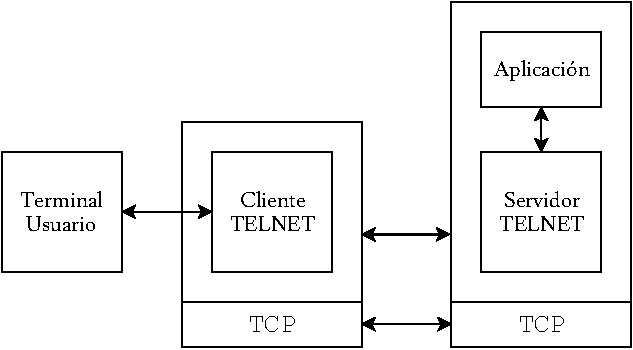
\includegraphics[page=1,scale=0.6]{TELNETDiag.pdf}
\caption{Esquema de funcionamiento de TELNET}
\end{figure}

\section*{SMPT (Simple Mail Transfer Protocol)}
Administra la transferencia de mensajes del sistema de correo de una computadora hacia otro sistema de correo remoto. Acepta correo local.
\subsection*{Funciones}
\begin{itemize}
\item El cliente opera con el inicio de la transferencia del correo hacia otro sistema.
\item El servidor esta relacionado con el correo que se recibe en el exterior.
\end{itemize}
El sistema de correo local asigna a cada usuario una casilla, en la que pueda depositar o recuperar el correo. Para poder llevar a cabo la entrega del correo es necesario:
\begin{itemize}
\item \textbf{Parte Local:} Es el nombre del usuario y es unico solo dentro del sistema de correo local.
\item \textbf{Parte Global:} Es la identidad del computador que debe ser unica dentro del internet.
\end{itemize}
\begin{figure}[H]
\centering
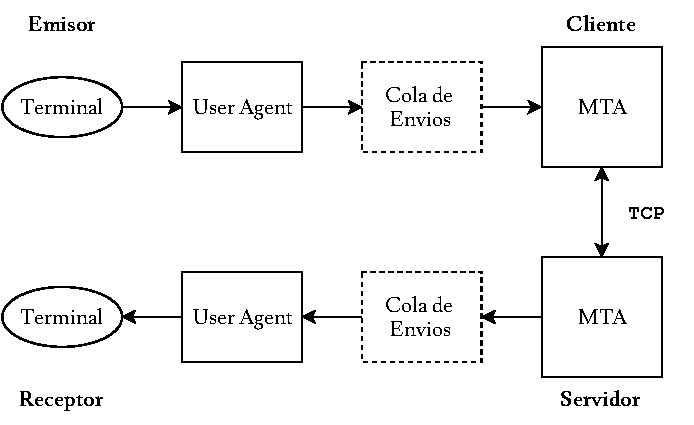
\includegraphics[page=1,scale=0.7]{SMTP.pdf}
\caption{Esquema de funcionamiento de SMTP}
\end{figure}
Cuando un cliente establece una conexión con el servidor SMTP, espera a que este envíe un mensaje ``Service Ready'' o ``Service not Avaiable''. Se envía un \texttt{HELLO} desde el cliente y con ellos el servidor se identifica, esto puede usarse para comprobar si se conectó. \\${ }$\\
El cliente comienza la transacción del correo con \texttt{MAIL FROM}, se puede pasar como argumento la dirección del correo al que el servidor notificará. \\${ }$\\
Luego, el servidor verifica si el origen es válido (\texttt{OK}).
\begin{itemize}
\item Ya le hemos dicho al servidor que queremos mandar un correo, hay que comunicarle a quien. La orden \texttt{RCPT TO}. Se puede enviar tantas veces como queramos.
\item Por cada uno el destinatario responde \texttt{OK} o ``No such user here''.
\item Una vez enviados a todos la \texttt{RCPT} el cliente envia una orden \texttt{DATA} para indicar que  a continuación se envían los contenidos del mensaje.
\item Una vez finalizado se termina con \texttt{CRLF OK} o mensaje de error.
\item Tras el envio el cliente si no tiene que enviar mas correos, da la orden \texttt{QUIT}. 
\end{itemize}